\documentclass{beamer}
\usetheme{afm}

\title{Interest Rate Derivatives}
\author{\href{mailto:matteo.sani@unisi.it}{Matteo Sani}}

\begin{document}
\begin{frame}[plain]
	\maketitle
\end{frame}

\begin{frame}{Interest Rate Swaps}
	\begin{itemize}
		\item \emph{Interest rate swaps} (IRS) consist of a floating leg and a fixed leg. The contract parameters are:
		\begin{itemize}
		\item start date $d_0$;
		\item notional $N$;
		\item fixed rate $K$;
		\item floating rate tenor;
		\item maturity.
		\end{itemize}
		\item \emph{Floating leg}: pays the reference IBOR fixing at a frequency equal to the index tenor (e.g. an IRS on a 3-month EURIBOR will pay coupons every three months).
		\item \emph{Fixed leg}: pays a predetermined cash flow at annual frequency (for simplicity only consider maturities multiples of 1 year).
	\end{itemize}
\end{frame}

\begin{frame}{IRS Valuation}
	\begin{itemize}
		\item The NPV of the fixed leg is calculated as follows:
		\begin{equation*}
		\mathrm{NPV}_{\mathrm{fixed}}(d, K) = N\cdot K\cdot\sum_{i=1}^{n}D(d, d_{i}^{\mathrm{fixed}})
		\end{equation*}
		\item While the NPV of the floating leg is:
		\begin{equation*}
			\mathrm{NPV}_{\mathrm{float}}(d, F) = N\cdot\sum_{i=1}^{m}F(d, d_{j-1}^{\mathrm{float}}, d_{j}^{\mathrm{float}}) \cdot \tau
\cdot D(d, d_{i}^{\mathrm{float}})
		\end{equation*}
		where $d_i^{\mathrm{fixed}}, d_i^{\mathrm{float}}$ are the payment dates, $d$ the pricing date, $D(d, d')$ the discount factor between $d$ and $d'$, $F(d, d', d'')$ the forward rate and $\tau = \frac{d_{j}^{\mathrm{float}}-d_{j-1}^{\mathrm{float}}}{360}$ the tenor.		
		\item Therefore the NPV of the swap (seen from the point of view of the counter-party which receives the floating leg) is
		\begin{equation*}
			\mathrm{NPV}(d, F, K) = \mathrm{NPV}_{\mathrm{float}}(d,F) - \mathrm{NPV}_{\mathrm{fixed}}(d,K)
		\end{equation*} 
	\end{itemize}
\end{frame}
	
\begin{frame}{IRS Valuation}
	\begin{itemize}	
	\item It's actually more convenient to express the NPV as a function of the \emph{swap rate} $S$.
	\item $S$ is the value of $K$ which makes $\mathrm{NPV}=0$ or 		$\mathrm{NPV}_{\mathrm{fixed}}(d, S) = \mathrm{NPV}_{\mathrm{float}}(d, F)$.
	\begin{equation*}
		\begin{gathered}
		N\cdot S\cdot\sum_{i=1}^{n}D(d, d_{i}^{\mathrm{fixed}}) = N\cdot\sum_{i=1}^{m}F(d, d_{j-1}^{\mathrm{float}}, d_{j}^{\mathrm{float}}) \cdot\tau\cdot D(d, d_{i}^{\mathrm{float}})\\
		S=\frac{\sum_{i=1}^{m}F(d, d_{j-1}^{\mathrm{float}}, d_{j}^{\mathrm{float}}) \cdot \tau\cdot D(d, d_{i}^{\mathrm{float}})}{\sum_{i=1}^{n}D(d, d_i^{\mathrm{fixed}})}
		\end{gathered}
	\end{equation*}
	\item Once calculated $S$, we can write:
	\begin{align*}
	&\mathrm{NPV} = \mathrm{NPV}_{\mathrm{float}}(d, F) - \mathrm{NPV}_{\mathrm{fixed}}(d, K) = \overbrace{\mathrm{NPV}_{\mathrm{float}}(d, F) - \mathrm{NPV}_{\mathrm{fixed}}(d, S)}^{\mathrm{=\;0}} + \\& + \mathrm{NPV}_{\mathrm{fixed}}(d, S) - \mathrm{NPV}_{\mathrm{fixed}}(d, K) = N\cdot(S-K)\cdot\underbrace{\sum_{i=1}^{n}D(d, d_{i}^{\mathrm{fixed}})}_{\mathrm{annuity}}
	\end{align*}
	\end{itemize}
\end{frame}

\begin{frame}{Interest Rate Swaptions}
	\begin{itemize}
		\item \emph{Swaptions} (Swap-options) are the equivalent of European options for the interest rate markets.
		\item They give the holder the right but not the obligation, at the exercise date $d_{ex}$, to enter into an Interest Rate Swap at a pre-determined fixed rate.
		\item The holder will choose to exercise the option only if the NPV of the underlying swap at $d_{ex}$ will be positive.
		\item From the IRS NPV expression, we can determine the payoff of the swaption 
		\begin{equation*}
		N\cdot \mathrm{max}(0, S(d_{\mathrm{ex}}) - K)\cdot\sum D(d, d_i^{\mathrm{fixed}})
		\end{equation*}
		\item In order to valuate the swaption the key point is to estimate $S(d_{\mathrm{ex}})$. 
		\item It will be shown with two alternative approaches.
	\end{itemize}
\end{frame}

\begin{frame}{Swaption Price with Black-Scholes}
    \begin{itemize}	
    \item First we'll use a generalization of the Black-Scholes formula for swaptions:
    \begin{equation*}
    \mathrm{NPV} = N\cdot A\cdot [S \Phi(d_+) - K\Phi(d_-)]
    \end{equation*}
    where $\Phi$ represents the cumulative distribution function of the normal distribution
    \begin{gather*}
    d_{\pm} = \frac{\mathrm{log}(\frac{S}{K}) \pm \frac{1}{2}\sigma^{2}T}{\sigma\sqrt{T}}\qquad(\sigma~\textrm{is the volatility of the swap rate})\\
    A =\sum_{i=1}^{p}D(d, d_{i}^{\mathrm{fixed}})\qquad\mathrm{(annuity})
    \end{gather*}
    \end{itemize}
\end{frame}

\begin{frame}{Swaption Price with Monte Carlo}
    \begin{itemize}
    \item An alternative approach is to assume that the swap rate $S$ evolves following a log normal process.
    \item Its distribution at the exercise date $S(d_{\mathrm{ex}})$ is
    \begin{equation*}
    S(d)\mathrm{exp}\left[-\frac{1}{2}\sigma^{2}T+\sigma\sqrt{T}\mathcal{N}(0,1)\right]	
    \end{equation*} 
	notice that the \emph{drift} rate in the evolution is zero.
    \item To simulate the swap rate we can:
    \begin{enumerate}
    \item sample $n$ times from the normal distribution $\mathcal{N}(0, 1)$ and calculate $S(d_{\mathrm{ex}})$ in different scenrios;
    \item evaluate the underlying swap's NPV at the exercise date, and consequently the swaption's payoff, for each scenario;
    \item take the average of these values to get the final estimate.
  	\end{enumerate} 
  	\item Further the 95\% confidence level for the swaption simulation can be calculated to compare with the BS result.
    \end{itemize}
\end{frame}

\begin{frame}{Credit Curves}
\begin{itemize}
    \item A \emph{credit event} can be a default, the failure to make payments, the issuer entering into bankruptcy proceedings, or the occurence of other legal events\dots (for simplicity credit event = default).
    \item \emph{Non-default probability} or \emph{survival probability} ($P_{\textrm{sur}}$): probability that the issuer of a contract will not suffer a credit event before a given date. 
    \item Note that non-default probability is a \emph{cumulative probability} since refers to a certain time horizon. 
    \item Just like a discount curve is a way of representing a set of discount factors, \emph{credit curves} are a way of representing survival probabilities.
\end{itemize}
\end{frame}

\begin{frame}{Hazard Rate}
	\begin{itemize}
		\item \emph{Hazard rate} measures the instantaneous probability of a company defaulting \emph{conditioned} on it not having defaulted until that moment.
		\item Hazard rate is often called a \emph{conditional failure rate} since is a direct application of the conditional probability concept (i.e. tells "how should you update probabilities of events when there is additional information available"). 
		\begin{equation*}
		\lambda(t) = -\cfrac{dP_{\textrm{sur}}}{dt}\cfrac{1}{P_{\textrm{sur}}(t_0, t)}
		\end{equation*}
		where the minus sign derives from the fact that $P_{\textrm{sur}}$ is a \emph{non} default probability while the hazard rate is defined in terms of the probability of default $P_{\textrm{def}}$.
	\end{itemize}
\end{frame}

\begin{frame}{Hazard Rate}
	\begin{itemize}
		\item Given the hazard rate the survival probability can be determined as:
		\begin{gather*}
		\lambda(t) = -\cfrac{1}{dt}\cdot\cfrac{dP_{\textrm{sur}}}{P_{\textrm{sur}}} = -\cfrac{d(\textrm{log}P_{\textrm{sur}})}{dt}\\[5pt]
		P_{\textrm{sur}}(t_0, t) = e^{-\int_{t_0}^{t}\lambda(s) ds}
		\end{gather*}
		
		\item For example a constant hazard rate results in the following probabilities:
		\begin{gather*}
			P_{\textrm{sur}}(t_0, t) = e^{-\lambda (t-t_0)}\\
			P_{\textrm{def}}(t_0, t) = 1 - e^{-\lambda (t-t_0)}
		\end{gather*}
	\end{itemize}
\end{frame}

%\begin{frame}{Accuracy of Monte Carlo Simulation}
%Imagine you don't know the probability of getting two consecutive K from a deck: what can be concluded from the result of a single MC experiment ?
%\begin{block}{Central Limit Theorem}    
%If $Y_1, Y_2,\dots, Y_n$ are $n$ random samples from a distribution $Y$ with true mean $\mu$ and variance $\sigma^{2}$, then when $n$ is sufficiently large, 
%\begin{equation*}
%\mu_n = \cfrac{1}{n}\sum_i^n Y_i \approx \mathcal{N}(\mu, \sigma^2/n)
%\end{equation*}
%has approximately a normal distribution $\mathcal{N}(\mu, \sigma^2/n)$. 
%
%This means that if ones repeats a MC experiment (changing the seed of the random number generator) she should obtain results normally distributed around the \emph{true} value $\mu$.
%\end{block}
%\end{frame}
%
%\begin{frame}{Confidence Interval}
%\begin{itemize}
%\item Since
%\begin{equation*}
%\mu_n \approx \mathcal{N}(\mu, \sigma^2/n)\implies \mu_n - \mu \approx \mathcal{N}(0, \sigma^2/n)
%\end{equation*}
%we can define an interval such that there is a given probability to find $\mu$ in there.
%\begin{columns}
%\column{0.5\linewidth}
%\begin{equation*}
%P\left(\mu_n - 1.96\frac{\sigma}{\sqrt{n}}\le \mu \le \mu_n + 1.96\frac{\sigma}{\sqrt{n}}\right) = 0.95
%\end{equation*}
%\column{0.5\linewidth}
%\begin{figure}[h]
%    \begin{center}
%    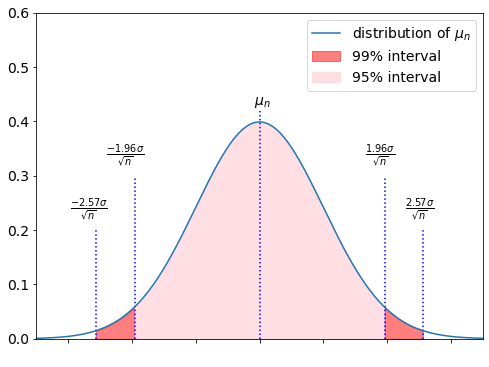
\includegraphics[width=0.8\linewidth]{confidence_interval_pink}
%    \end{center}
%\end{figure}    
%\end{columns}
%\item This is the \emph{95\% confidence interval} since pink area is 95\% of the area under the Gaussian.
%\item Repeating many times a simulation, the fraction of confidence intervals containing the true $\mu$ would tend toward 95\%.
%\end{itemize}
%\end{frame}
%
%\begin{frame}[fragile]{Confidence Interval}
%The most common intervals are 99\% and 95\% confidence levels and are respectively defined as $\pm \cfrac{2.57\sigma}{\sqrt{n}}$ and $\pm \cfrac{1.96\sigma}{\sqrt{n}}$. 
%\begin{ipython}
%import numpy as np
%
%cl = 1.96*np.std(r)/np.sqrt(experiments)
%print (f"{np.mean(r):.6f} +- {cl:.6f} @ 95% confidence level")
%# 0.007689 +- 0.000054 @ 95% confidence level
%\end{ipython}
%\end{frame}
%
%\begin{frame}[fragile]{Standard Deviation of the Mean}
%\begin{itemize}
%\item To get further information about the precision of our estimate $\mu_n$, or about the accuracy of the Monte Carlo simulation in general, we can use the standard deviation of the sampled mean. 
%\item Assuming statistical independence of the values in the sample, the standard deviation of the mean is 
%\begin{equation*}
%\sigma _{\text{mean}}={\frac {1}{\sqrt {n}}}\sigma
%\end{equation*}
%where $n$ is the number of observations in the sample used to estimate the mean. 
%
%\begin{ipython}
%print (f"{np.mean(r):.6f} +- {np.std(r)/np.sqrt(experiments):.6f}")
%# 0.007689 +- 0.000028
%\end{ipython}
%\item To get one more digit of accuracy (i.e. an error one tenth as large) requires a $\times100$ simulations.
%\item To get three more digits of accuracy requires one million times as much computation: \emph{running 10000 above experiments ($\times10$ more) gives an error 3 times smaller (from 2.8e-5 to about 9e-6)}.
%\end{itemize}
%\end{frame}
%
%\begin{frame}{Stochastic Processes}
%\begin{itemize}
%\item \emph{Deterministic process}: all data necessary to predict the system development with 100\% certainty is available.
%\item \emph{Stochastic or random process}: exhibits behaviors that cannot be described by a deterministic model, is a \emph{noisy} process where uncertainty needs to be modeled
%   \begin{itemize}
%    \item it is a collection of random variables indexed by some set (usually time);
%    \item each random variable of the stochastic process is uniquely associated with an element in the set. 
%    \end{itemize}
%\begin{figure}[h]
%    \begin{center}
%    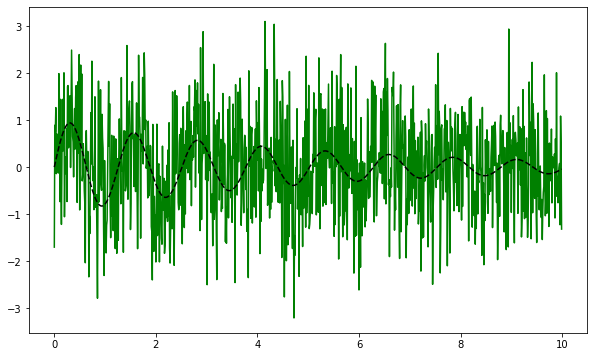
\includegraphics[width=0.5\linewidth]{stochastic_process}
%    \end{center}
%\end{figure}        
%\end{itemize}
%\end{frame}
%
%\begin{frame}{Stochastic Processes}
%\begin{itemize}
%\item Stochastic processes are described by \emph{stochastic differential equation (SDE)}:
%\begin{equation*}
%dX(t) = \mu(t,X(t)) dt + \sigma(t,X(t)) dW(t) = \underbrace{\mu(t,X(t))dt}_{\textrm{deterministic}} + \underbrace{\sigma(t,X(t)) \mathcal{N}(0,1)\sqrt{dt}}_{\textrm{stochastic}}
%\end{equation*}
%\item The mean of $dW$ is zero and its variance is $dt$
%   \begin{itemize}
%    \item the standard deviation grows with the square root of time: $W(t) - \mathcal{N}( 0, t )$ because each $dW$ is distributed like independent standard Gaussian.
%    \end{itemize}
%\end{itemize}
%\begin{figure}[h]
%    \begin{center}
%    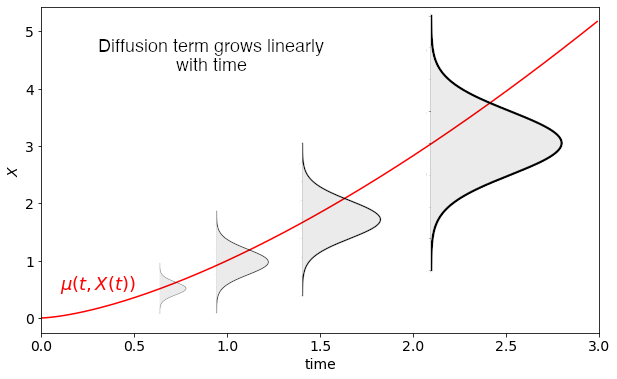
\includegraphics[width=0.50\linewidth]{brownian_process}
%    \end{center}
%\end{figure}        
%\end{frame}
%
%\begin{frame}{Geometric Brownian Motion}
%\begin{itemize}
%\item Stock prices changes as a result of the random fluctuations given by the trades. The relative change in its price in a period $dt$ can be decomposed into two parts:
%\begin{itemize}
%    \item \emph{deterministic}, the expected return from the stock hold during the time period $dt$ ($\mu S_tdt$);
%    \item \emph{stochastic} which reflects the random changes of the market (e.g. as a response to external effects such as unexpected news). A reasonable assumption is to take this contribution proportional to the stock ($\sigma S_t dW_t$).
%\end{itemize}
%\begin{equation*}
%dS_t = \mu S_tdt + \sigma S_tdW_t;\quad\frac{dS_t}{S_t} = d\textrm{log}(S_t) = \mu dt + \sigma dW_t 
%\end{equation*}
%\item The solution of this SDE can be derived by applying the It$\hat{o}$'s formula (full derivation in the notes).
%\begin{equation*}
%S_t = S_{t-1}e^{\big(\mu - \frac{1}{2}\sigma^2\big)dt + \sigma Z\sqrt{dt}}
%\end{equation*}
%\end{itemize}
%\end{frame}
%
%\begin{frame}{Geometric Brownian Motion}
%\begin{itemize}
%\item The change in $\textrm{log} S_t$ has a constant \emph{drift} $\mu - \frac{1}{2}\sigma^2$ and a constant variance rate $\sigma^2$ (remember that $Z=\mathcal{N}(0,1)$) therefore $\textrm{log} S_t$ at some time $T$ is normally distributed with:
%\begin{equation*}
%\textrm{log}\left(\cfrac{S_t}{S_{t-1}}\right) = \left(\mu - \frac{1}{2}\sigma^2\right)dt + \sigma Z\sqrt{dt} \approx\mathcal{N}\left[\left(\mu-\frac{\sigma^2}{2}\right)T, \sigma^2 T\right]
%\end{equation*}
%\end{itemize}
%\begin{block}{}
%A variable whose logarithm is normally distributed is said to be \emph{log-normal}, lognormality is important because ensures a stock price will never be negative.
%Looking at the initial $dS$ equation we had that:
%\begin{equation*}
%dS_t = \mu S_tdt + \sigma S_tdB_t
%\end{equation*}
%which shows that the closer is $S_t$ to 0 the smaller is the $dS$ variation (so it will never go below 0).
%\end{block}
%%\begin{figure}[h]
%%    \begin{center}
%%    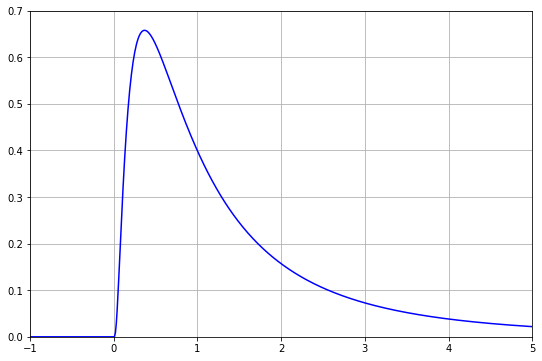
\includegraphics[width=0.7\linewidth]{lognormal}
%%    \end{center}
%%\end{figure}        
%\end{frame}
%
%\begin{frame}{Simulating SDE}
%\begin{itemize}
%\item  Consider the generic SDE
%\begin{equation*}
%dX(t) = \mu(t,X(t))dt + \sigma(t,X(t))dW(t)
%\end{equation*}
%the simulation of $X(t)$ is done as follows.
%\item Starting from the value of $X(t_i)$ compute $X(t_{i+1})$ using the given SDE by setting $\Delta t = t_{i+1} - t_{i}$, and sampling from a standard normal $\mathcal{N}(0,1)$
%\begin{equation*}
%X(t_{i+1}) = X(t_i) + \mu(t_i,X(t_i))\Delta t + \sigma(t_i,X(t_i))\sqrt{\Delta t}\mathcal{N}(0,1)
%\end{equation*}
%\end{itemize}
%\end{frame}
%
%\begin{frame}{Remark on Stochastic Processes}
%\begin{itemize}
%\item Whenever we want to estimate a quantity involving stochastic processes we have to compute an expectation $\mathbb{E}[f(X)]$.
%\item This means that we have to average the value of $f(X)$ among all the possible realizations of $X$ taking into account the probability associated to each path.
%\item Monte Carlo simulation is a way of estimate an expectation: 
%\begin{enumerate}
%\item simulate as many $X$ realization as possible;
%\item for each simulation compute $f(X)$;
%\item average the results to estimate $\mathbb{E}[f(X)]$.
%\end{enumerate}
%\end{itemize}
%\end{frame}

\end{document}
